% Intended LaTeX compiler: pdflatex
\documentclass[../main]{subfiles}

\def\Hk#1{\mathrm{H}^{#1}_{\text{dR}}}
\def\Toro{\mathds{T}}
\def\ToroBucato{\tilde{\Toro}}


\begin{document}

\section{Coomologia delle superfici topologiche compatte orientabili}
\label{sec:orgd09f4df}
\begin{thm}
Se \(\Sigma_{g}\) è la \href{20251230172241-superficie_topologica.org}{superficie topologica} \href{20250103163701-spazio_topologico_compatto.org}{compatta} \href{20251223152054-varieta_differenziabile_orientabile.org}{orientabile} di genere \(g\), allora la \href{20251115172442-gruppo_di_coomologia_di_de_rham.org}{Coomologia di De Rham} è\footnote{Vedi ``\href{20241213095808-somma_diretta.org}{Somma Diretta}''}
\begin{equation*}
\Hk{k}(\Sigma_{g}) \cong \begin{cases}
\R & k = 0,2\\
\R^{g} \oplus \R^{g} & k = 1\\
0 & \text{altrimenti}
\end{cases}
\end{equation*}
dove ``\(\cong\)'' è un \href{20250113125833-isomorfismo_tra_spazi_vettoriali.org}{isomorfismo}.
\label{thm:coomsigmag}
\end{thm}
\begin{lem}
La coomologia del toro bucato, \(\ToroBucato \coloneqq \Toro \setminus\set{\text{punto}}\) è
\begin{equation*}
\Hk{k}(\ToroBucato) \cong %
\begin{cases}
\R & k = 0\\
\R^{2} & k = 1\\
0 & k\ge 0
\end{cases}
\end{equation*}
\label{lem:coomtorobuc}
\end{lem}
\begin{proof}
Dato il Toro \(\Toro\), \href{20251115190941-coomologia_del_toro.org}{di cui si conosce la coomologia}\footnote{Si ha che
\begin{equation*}
\Hk{k}(\Toro) \cong
\begin{cases}
\R & k = 0,2\\
\R^{2} & k=1
\end{cases}
\end{equation*}}, si considera:
\begin{equation*}
     \Toro = \ToroBucato \cup D
\end{equation*}
dove \(\ToroBucato = \Toro\setminus\set{p}\) e \(D\) è un intorno aperto attorno a \(p\), omotopo a \(\R^{2}\), \href{20251115173712-coomologia_di_de_rham_di_r2.org}{di cui si conosca le coomologia}\footnote{Si ha che
\begin{equation*}
\Hk{k}(\R^{2}) \cong %
\begin{cases}
\R & k=0\\
O & k\neq 0
\end{cases}
\end{equation*}}. Si noti che \(\ToroBucato\cap D\) è omotopo a \(\mathds{S}^{1}\), \href{20251115184223-coomologia_della_circonferenza.org}{di cui si conosce la coomologia}\footnote{Si ha che
\begin{equation*}
\Hk{k}(\mathds{S}^{1}) \cong %
\begin{cases}
\R & k = 0,1\\
0 & k \ge 2
\end{cases}
\end{equation*}}. Si scrive quindi \href{20251115183635-teorema_di_mayer_vietoris_in_coomologia.org}{Mayer-Vietoris}:
\begin{equation*}
\begin{tikzcd}[column sep=small]
        0 & {\Hk{0}(\Toro)} & {\Hk{0}(\ToroBucato)\oplus\Hk{0}(D)} & {\Hk{0}(\ToroBucato \cap D)} \\
        & {\Hk{1}(\Toro)} & {\Hk{1}(\ToroBucato)\oplus\Hk{1}(D)} & {\Hk{1}(\ToroBucato \cap D)} \\
        & {\Hk{2}(\Toro)} & {\Hk{2}(\ToroBucato)\oplus\Hk{2}(D)} & {\Hk{2}(\ToroBucato \cap D)} & 0
        \arrow[from=1-1, to=1-2]
        \arrow[from=1-2, to=1-3]
        \arrow[from=1-3, to=1-4]
        \arrow[from=1-4, to=2-2]
        \arrow[from=2-2, to=2-3]
        \arrow[from=2-3, to=2-4]
        \arrow[from=2-4, to=3-2]
        \arrow[from=3-2, to=3-3]
        \arrow[from=3-3, to=3-4]
        \arrow[from=3-4, to=3-5]
\end{tikzcd}
\end{equation*}
Si possono semplificare alcuni termini:
\begin{itemize}
\item siccome tutti gli spazi sono connessi, \href{20251115174538-0_gruppo_di_coomologia_di_de_rham_di_una_varieta_connessa.org}{ogni \(\Hk{0}\) è isomorfo a \(\R\)} (in particolare, \(\boxed{\Hk{0}(\ToroBucato) \cong \R}\));
\item siccome \(\ToroBucato\) è \href{20251223152054-varieta_differenziabile_orientabile.org}{orientabile} ma \href{20250103163701-spazio_topologico_compatto.org}{non compatta}, \href{20251117121206-coomologia_in_dimensione_massima.org}{allora} \(\boxed{\Hk{2}(\ToroBucato) = 0}\);
\item si sostituiscono gli \(\Hk{k}(D) \cong \Hk{k}(\R^{2})\) e \(\Hk{k}(\ToroBucato\cap D)\cong \Hk{k}(\mathds{S}^{1})\), nonché gli elementi della coomologia di \(\Toro\).
\end{itemize}
La successione esatta è necessaria solo più per calcolare \(\Hk{1}(\ToroBucato)\):
\begin{equation*}
\begin{tikzcd}[column sep=small]
        0 & \R & {\R\oplus\R} & \R \\
        & {\R^2} & {\Hk{1}(\ToroBucato)} & \R \\
        & \R & 0 & 0 & 0
        \arrow[from=1-1, to=1-2]
        \arrow[from=1-2, to=1-3]
        \arrow[from=1-3, to=1-4]
        \arrow[from=1-4, to=2-2]
        \arrow[from=2-2, to=2-3]
        \arrow[from=2-3, to=2-4]
        \arrow[from=2-4, to=3-2]
        \arrow["\beta"', from=3-2, to=3-3]
        \arrow[from=3-3, to=3-4]
        \arrow[from=3-4, to=3-5]
\end{tikzcd}
\end{equation*}
(\emph{Non dimostrato}: \(\Hk{1}(\ToroBucato)\) ha dimensione finita). Utilizzando la \href{20251115182133-successione_di_spazi_vettoriali_esatta.org}{somma alterna delle dimensioni}, si ottiene che
\begin{equation*}
     -1+2-1+2-\dim \Hk{1}(\ToroBucato) +1 -1 = 0
\end{equation*}
ovvero \(\dim \Hk{1}(\ToroBucato) = 2\), \(\boxed{\Hk{1}(\ToroBucato) \cong \R^{2}}\).
\end{proof}
\begin{proof}
(Del Teorema~\ref{thm:coomsigmag})
\uline{Caso \(k=0\)}: siccome \(\Sigma_{g}\) è \href{20250103165325-spazio_topologico_connesso.org}{connessa}, \href{20251115174538-0_gruppo_di_coomologia_di_de_rham_di_una_varieta_connessa.org}{allora} \(\boxed{\Hk{0}(\Sigma_{g}) = \R}\).

\uline{Caso \(k=2\) e \(k\ge 2\)}: \(\Sigma_{g}\) è una \href{20250113115909-struttura_differenziabile.org}{varietà differenziabile} di dimensione \(2\).
\begin{itemize}
\item per ogni \(k>2\): \(\Hk{k}(\Sigma_{g}) = 0\), per questione di dimensione;
\item per \(k=2\): siccome \(\Sigma_{g}\) è compatta e orientabile, allora (\href{20251117121206-coomologia_in_dimensione_massima.org}{Coomologia in dimensione massima})
\begin{equation*}
  \boxed{\Hk{2}(\Sigma_{g}) \cong \R}
\end{equation*}
\end{itemize}

\uline{Caso \(k=1\)}: Consideriamo \(\Sigma_{g}\) rappresentato in Figura~\ref{fig:multitoro_normale}: possiamo dividerlo nei due insiemi \(U,V\), rappresentati in Figura~\ref{fig:multitoro_UeV}:
\begin{itemize}
\item \(U\) è \href{20250124155008-spazi_topologici_omotopicamente_equivalenti.org}{omotopo} alla superficie \(\tilde{\Sigma}_{g-1} \coloneqq \Sigma_{g-1} \setminus \set{\text{punto}}\);
\item \(V\) è omotopo a \(\ToroBucato \coloneqq \Toro \setminus \set{\text{punto}}\), dove \(\Toro\) è il \href{20250113125113-toro.org}{Toro}.
\item \(U\cap V\) è omotopo a \(\mathds{S}^1\), come si vede in Figura~\ref{fig:multitoro_UcapV}.
\end{itemize}

Siccome si vuole utilizzare la \href{20251115183635-teorema_di_mayer_vietoris_in_coomologia.org}{sequenza di Mayer-Vietoris}, (sfruttando l'\href{20251223145901-teorema_di_invarianza_omotopica_per_la_coomologia_di_de_rham.org}{invarianza della coomologia per omotopia}) è necessario calcolare la coomologia di \(\tilde{\Sigma}_{g-1}\). Si procede per induzione
\begin{itemize}
\item \uline{Caso base}: \(\Sigma_{1} = \Toro\), è verificato.
\item \uline{Ipotesi induttiva}: si supponga vera l'ipotesi per \(\Sigma_{g-1}\):
\begin{equation*}
\Hk{1}(\Sigma_{g-1}) \cong \R^{g-1} \oplus \R^{g-1}
\end{equation*}
Si vuole dimostrare la tesi per \(\Sigma_{g}\). Si procede scrivendo la successione di Mayer-Vietoris, utilizzando \(U\) e \(V\) come sopra.
\begin{equation*}
\begin{tikzcd}[column sep=small]
        0 & {\Hk{0}(\Sigma_g)} & {\Hk{0}(U)\oplus \Hk{0}(V)} & {\Hk{0}(U\cap V)} \\
        & {\Hk{1}(\Sigma_g)} & {\Hk{1}(U)\oplus \Hk{1}(V)} & {\Hk{1}(U\cap V)} \\
        & {\Hk{2}(\Sigma_g)} & {\Hk{2}(U)\oplus \Hk{2}(V)} & {\Hk{2}(U\cap V)} & 0
        \arrow[from=1-1, to=1-2]
        \arrow[from=1-2, to=1-3]
        \arrow[from=1-3, to=1-4]
        \arrow[from=1-4, to=2-2]
        \arrow[from=2-2, to=2-3]
        \arrow[from=2-3, to=2-4]
        \arrow[from=2-4, to=3-2]
        \arrow[from=3-2, to=3-3]
        \arrow[from=3-3, to=3-4]
        \arrow[from=3-4, to=3-5]
\end{tikzcd}
\end{equation*}
Sostituendo utilizzando le considerazioni sull'omotopia:
\begin{equation*}
\begin{tikzcd}[column sep=small]
        0 & {\Hk{0}(\Sigma_g)} & {\Hk{0}(\tilde{\Sigma}_{g-1})\oplus \Hk{0}(\ToroBucato)} & {\Hk{0}(\mathds{S}^1)} \\
        & {\Hk{1}(\Sigma_g)} & {\Hk{1}(\tilde{\Sigma}_{g-1})\oplus \Hk{1}(\ToroBucato)} & {\Hk{1}(\mathds{S}^1)} \\
        & {\Hk{2}(\Sigma_g)} & {\Hk{2}(\tilde{\Sigma}_{g-1})\oplus \Hk{2}(\ToroBucato)} & {\Hk{2}(\mathds{S}^1)} & 0
        \arrow[from=1-1, to=1-2]
        \arrow[from=1-2, to=1-3]
        \arrow[from=1-3, to=1-4]
        \arrow[from=1-4, to=2-2]
        \arrow[from=2-2, to=2-3]
        \arrow[from=2-3, to=2-4]
        \arrow[from=2-4, to=3-2]
        \arrow[from=3-2, to=3-3]
        \arrow[from=3-3, to=3-4]
        \arrow[from=3-4, to=3-5]
\end{tikzcd}
\end{equation*}
\begin{itemize}
\item Tutte le superfici in gioco sono connesse, quindi \(\Hk{0} \cong \R\);
\item Si conoscono la coomologia \href{20251115184223-coomologia_della_circonferenza.org}{di \(\mathds{S}^{1}\)} e \(\ToroBucato\)\footnote{Vedi il Lemma~\ref{lem:coomtorobuc}}, nonché le coomologie di dimensione \(0\) e \(2\) si \(\Sigma_{g}\);
\item \(\tilde{\Sigma}_{g-1}\) è una superficie orientabile non compatta, e \href{20251117121206-coomologia_in_dimensione_massima.org}{quindi} \(\Hk{2}(\tilde{\Sigma}_{g-1}) \cong 0\).
\end{itemize}
Resta quindi:
\begin{equation*}
\begin{tikzcd}[column sep=small]
        0 & \R & {\R\oplus \R} & \R \\
        & {\Hk{1}(\Sigma_g)} & {\Hk{1}(\tilde{\Sigma}_{g-1})\oplus \R^2} & \R \\
        & \R & 0 & 0 & 0
        \arrow[from=1-1, to=1-2]
        \arrow[from=1-2, to=1-3]
        \arrow[from=1-3, to=1-4]
        \arrow[from=1-4, to=2-2]
        \arrow[from=2-2, to=2-3]
        \arrow[from=2-3, to=2-4]
        \arrow[from=2-4, to=3-2]
        \arrow[from=3-2, to=3-3]
        \arrow[from=3-3, to=3-4]
        \arrow[from=3-4, to=3-5]
\end{tikzcd}
\end{equation*}
Utilizzando la \href{20251115182133-successione_di_spazi_vettoriali_esatta.org}{somma alterna delle dimensioni} si ottiene:
\begin{align*}
  0 &= 1 - 2 + 1 - \dim \Hk{1}(\Sigma_{g}) + \dim \Hk{1}({\Sigma}_{g-1}) + 2 - 1 + 1\\
  \dim \Hk{1}(\Sigma_{g}) &= 1 - 2 + 1  + \dim \Hk{1}({\Sigma}_{g-1}) + 2 - 1 + 1 = %
  \dim \Hk{1}({\Sigma}_{g-1}) + 2. %
   \tag{$\star\star$}
\end{align*}

È qui che entra in gioco l'ipotesi induttiva. Se si considera \(\Sigma_{g-1} = A \cup B\), con \(A = \Sigma_{g-1} \setminus \set{q}\) e \(B\) intorno aperto di \(q\) omotopo a \(\R^{2}\), si ottiene che:
\begin{itemize}
\item \(\Hk{k}(A) \cong \Hk{k}(\tilde{\Sigma}_{g-1})\), in quanto sono omotopi, di cui si conoscono tutte le coomologie tranne \(\Hk{1}\):
\begin{equation*}
	\Hk{0}(\tilde{\Sigma}_{g-1}) \cong \R, \qquad \Hk{2}(\tilde{\Sigma}_{g-1}) = 0;
\end{equation*}

\item \(\Hk{k}(B) \cong \Hk{k}(\R^{2})\), \href{20251115173712-coomologia_di_de_rham_di_r2.org}{coomologia nota};

\item \(\Hk{k}(A \cap B) \cong \Hk{k}(\mathds{S}^{1})\), \href{20251115184223-coomologia_della_circonferenza.org}{coomologia nota}.
\end{itemize}

Scrivendo Mayer-Vietoris:
\begin{equation*}
\begin{tikzcd}[column sep=small]
        0 & {\Hk{0}(\Sigma_{g-1})} & {\Hk{0}(\tilde{\Sigma}_{g-1})\oplus\Hk{0}(\R^2)} & {\Hk{0}(\mathds{S}^1)} \\
        & {\Hk{1}(\Sigma_{g-1})} & {\Hk{1}(\tilde{\Sigma}_{g-1})\oplus\Hk{1}(\R^2)} & {\Hk{1}(\mathds{S}^1)} \\
        & {\Hk{2}(\Sigma_{g-1})} & {\Hk{2}(\tilde{\Sigma}_{g-1})\oplus\Hk{2}(\R^2)} & {\Hk{2}(\mathds{S}^1)} & 0
        \arrow[from=1-1, to=1-2]
        \arrow[from=1-2, to=1-3]
        \arrow[from=1-3, to=1-4]
        \arrow[from=1-4, to=2-2]
        \arrow[from=2-2, to=2-3]
        \arrow[from=2-3, to=2-4]
        \arrow[from=2-4, to=3-2]
        \arrow[from=3-2, to=3-3]
        \arrow[from=3-3, to=3-4]
        \arrow[from=3-4, to=3-5]
\end{tikzcd}
\end{equation*}

Per ipotesi induttiva si conoscono tutte le \(\Hk{k}(\Sigma_{g-1})\), e pertanto, sostituendo tutte le coomologie note:
\begin{equation*}
\begin{tikzcd}[column sep=small]
        0 & \R & {\R\oplus \R} & \R \\
        & {\R^{g-1} \oplus \R^{g-1}} & {\Hk{1}(\tilde{\Sigma}_{g-1})\oplus 0} & \R \\
        & \R & {0 \oplus 0} & 0 & 0
        \arrow[from=1-1, to=1-2]
        \arrow[from=1-2, to=1-3]
        \arrow[from=1-3, to=1-4]
        \arrow[from=1-4, to=2-2]
        \arrow[from=2-2, to=2-3]
        \arrow[from=2-3, to=2-4]
        \arrow[from=2-4, to=3-2]
        \arrow[from=3-2, to=3-3]
        \arrow[from=3-3, to=3-4]
        \arrow[from=3-4, to=3-5]
\end{tikzcd}
\end{equation*}
e facendo la \href{20251115182133-successione_di_spazi_vettoriali_esatta.org}{somma alterna delle dimensioni}:
\begin{equation*}
   \dim \Hk{1}(\tilde{\Sigma}_{g-1}) = -1+2-1+2(g-1)  +1 -1 = 2(g-1)
\end{equation*}
che, applicata in (\(\star\star\)):
\begin{equation*}
  \boxed{\Hk{1}(\Sigma_{g}) \cong \R^{g} \oplus \R^{g}}.%
  \qedhere
\end{equation*}
\end{itemize}
\end{proof}
\begin{figure}
\begin{equation*}
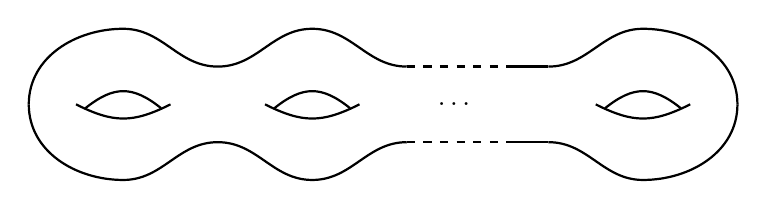
\begin{tikzpicture}[scale=1.2, line width=0.8pt]

    % Definizione corretta del comando \buco con 2 argomenti
    \newcommand{\buco}[2]{
        \draw (#1-0.5, #2) .. controls (#1-0.1, #2-0.2) and (#1+0.1, #2-0.2) .. (#1+0.5, #2);
        \draw (#1-0.4, #2-0.04) .. controls (#1-0.1, #2+0.2) and (#1+0.1, #2+0.2) .. (#1+0.4, #2-0.04);
    }

    % -- Parte Sinistra: Sigma_{g-1} senza un punto (U) --
    \draw (-4, 0) to[out=90, in=180] (-3, 0.8)
                  to[out=0, in=180] (-2, 0.4)
                  to[out=0, in=180] (-1, 0.8)
                  to[out=0, in=180] (0, 0.4); % Collo aperto a destra

    \draw (-4, 0) to[out=-90, in=180] (-3, -0.8)
                  to[out=0, in=180] (-2, -0.4)
                  to[out=0, in=180] (-1, -0.8)
                  to[out=0, in=180] (0, -0.4); % Collo aperto a destra

    \buco{-3}{0}
    \buco{-1}{0}

    % -- Parte Centrale: Tratteggio e sovrapposizione --
    \draw[dashed] (0, 0.4) -- (1.13, 0.4);
    \draw[dashed] (0, -0.4) -- (1.13, -0.4);


    % Puntini di sospensione per il genere generico
    \node at (0.5, 0) {$\dots$};

    % -- Parte Destra: Toro bucato (V) --
    \draw (1.13, 0.4) -- (1.5, 0.4);
    \draw (1.13, -0.4) -- (1.5, -0.4);

    \draw (1.5, 0.4) to[out=0, in=180] (2.5, 0.8)
                   to[out=0, in=90] (3.5, 0);

    \draw (1.5, -0.4) to[out=0, in=180] (2.5, -0.8)
                    to[out=0, in=-90] (3.5, 0);

    \buco{2.5}{0}

\end{tikzpicture}
\end{equation*}
\caption{\label{fig:multitoro_normale}La superficie \(\Sigma_{g}\)}
\end{figure}


\begin{figure}
\begin{equation*}
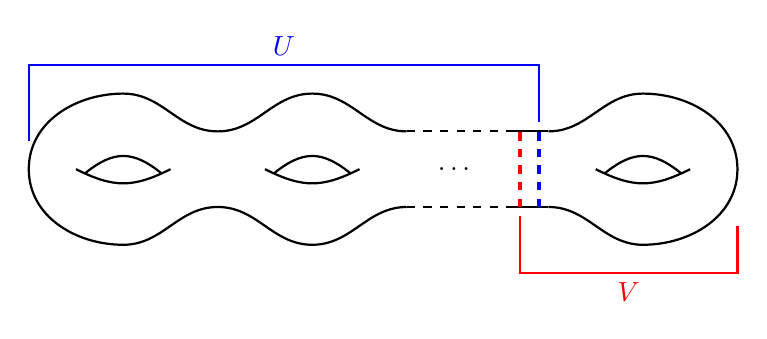
\begin{tikzpicture}[scale=1.2, line width=0.8pt]

    % Definizione corretta del comando \buco con 2 argomenti
    \newcommand{\buco}[2]{
        \draw (#1-0.5, #2) .. controls (#1-0.1, #2-0.2) and (#1+0.1, #2-0.2) .. (#1+0.5, #2);
        \draw (#1-0.4, #2-0.04) .. controls (#1-0.1, #2+0.2) and (#1+0.1, #2+0.2) .. (#1+0.4, #2-0.04);
    }

    % -- Parte Sinistra: Sigma_{g-1} senza un punto (U) --
    \draw (-4, 0) to[out=90, in=180] (-3, 0.8)
                  to[out=0, in=180] (-2, 0.4)
                  to[out=0, in=180] (-1, 0.8)
                  to[out=0, in=180] (0, 0.4); % Collo aperto a destra

    \draw (-4, 0) to[out=-90, in=180] (-3, -0.8)
                  to[out=0, in=180] (-2, -0.4)
                  to[out=0, in=180] (-1, -0.8)
                  to[out=0, in=180] (0, -0.4); % Collo aperto a destra

    \buco{-3}{0}
    \buco{-1}{0}

    % -- Parte Centrale: Tratteggio e sovrapposizione --
    \draw[dashed] (0, 0.4) -- (1.13, 0.4);
    \draw[dashed] (0, -0.4) -- (1.13, -0.4);


    % Puntini di sospensione per il genere generico
    \node at (0.5, 0) {$\dots$};

    % -- Parte Destra: Toro bucato (V) --
    \draw (1.13, 0.4) -- (1.5, 0.4);
    \draw (1.13, -0.4) -- (1.5, -0.4);

    \draw (1.5, 0.4) to[out=0, in=180] (2.5, 0.8)
                   to[out=0, in=90] (3.5, 0);

    \draw (1.5, -0.4) to[out=0, in=180] (2.5, -0.8)
                    to[out=0, in=-90] (3.5, 0);

    \buco{2.5}{0}

    \draw[red, line width=1.2pt, dashed] (1.2, -0.4) -- (1.2, 0.4);
    \draw[red] (1.2, -0.5) -- (1.2, -1.1) -- (3.5, -1.1) -- (3.5, -0.6);
    \node at (2.35,-1.3) {\textcolor{red}{\(V\)}};

    \draw[blue, line width=1.2pt, dashed] (1.4, -0.4) -- (1.4, 0.4);
    \draw[blue] (1.4, 0.5) -- (1.4, 1.1) -- (-4, 1.1) -- (-4, 0.3);
    \node at (-1.3,1.3) {\textcolor{blue}{\(U\)}};
\end{tikzpicture}
\end{equation*}
\caption{\label{fig:multitoro_UeV}Gli insiemi \(U\) e \(V\)}
\end{figure}

\begin{figure}
\begin{equation*}
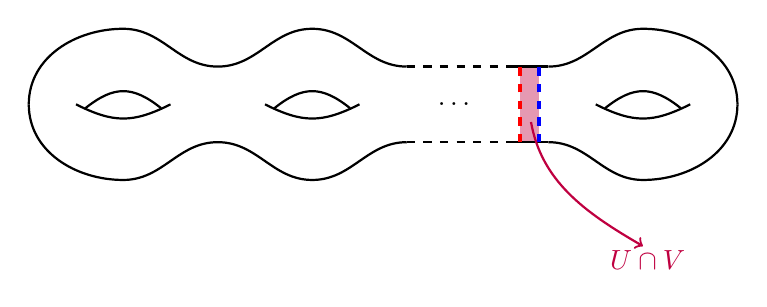
\begin{tikzpicture}[scale=1.2, line width=0.8pt]

    \fill[color=purple!40] (1.2, -0.4) rectangle (1.4, 0.4);

%    \fill[pattern=north west lines, pattern color=red] (1.2, -0.4) rectangle (1.4, 0.4);

    % Definizione corretta del comando \buco con 2 argomenti
    \newcommand{\buco}[2]{
        \draw (#1-0.5, #2) .. controls (#1-0.1, #2-0.2) and (#1+0.1, #2-0.2) .. (#1+0.5, #2);
        \draw (#1-0.4, #2-0.04) .. controls (#1-0.1, #2+0.2) and (#1+0.1, #2+0.2) .. (#1+0.4, #2-0.04);
    }

    % -- Parte Sinistra: Sigma_{g-1} senza un punto (U) --
    \draw (-4, 0) to[out=90, in=180] (-3, 0.8)
                  to[out=0, in=180] (-2, 0.4)
                  to[out=0, in=180] (-1, 0.8)
                  to[out=0, in=180] (0, 0.4); % Collo aperto a destra

    \draw (-4, 0) to[out=-90, in=180] (-3, -0.8)
                  to[out=0, in=180] (-2, -0.4)
                  to[out=0, in=180] (-1, -0.8)
                  to[out=0, in=180] (0, -0.4); % Collo aperto a destra

    \buco{-3}{0}
    \buco{-1}{0}

    % -- Parte Centrale: Tratteggio e sovrapposizione --
    \draw[dashed] (0, 0.4) -- (1.13, 0.4);
    \draw[dashed] (0, -0.4) -- (1.13, -0.4);


    % Puntini di sospensione per il genere generico
    \node at (0.5, 0) {$\dots$};

    % -- Parte Destra: Toro bucato (V) --
    \draw (1.13, 0.4) -- (1.5, 0.4);
    \draw (1.13, -0.4) -- (1.5, -0.4);

    \draw (1.5, 0.4) to[out=0, in=180] (2.5, 0.8)
                   to[out=0, in=90] (3.5, 0);

    \draw (1.5, -0.4) to[out=0, in=180] (2.5, -0.8)
                    to[out=0, in=-90] (3.5, 0);

    \buco{2.5}{0}

    \draw[red, line width=1.2pt, dashed] (1.2, -0.4) -- (1.2, 0.4);

    \draw[blue, line width=1.2pt, dashed] (1.4, -0.4) -- (1.4, 0.4);

% 2. ETICHETTA E FRECCIA U CAP V:
    % Definiamo un nodo per l'etichetta posizionato in basso a destra
    \node at (2.55, -1.65) {\textcolor{purple}{$U \cap V$}};

    % Disegniamo la freccia. 'shorten >=' fa fermare la punta poco prima del target.
    % Usiamo 'to[out=..., in=...]' per una freccia curva più elegante.
    \draw[<-, thick, purple, shorten >= 3pt] (2.5, -1.5) to[out=150, in=-80] (1.3, -0.1);
\end{tikzpicture}
\end{equation*}
\caption{\label{fig:multitoro_UcapV}L'insieme \(U\cap V\)}
\end{figure}
\end{document}
